\documentclass[final,hyperref={pdfpagelabels=false}]{beamer}
\mode<presentation>
{
  \usetheme{UNM}
}
  \usepackage{times}
  \usepackage{bm}
  \usepackage{ragged2e}
  \usepackage[numbers]{natbib}
  \usepackage{amsmath, amsthm, amssymb, latexsym}
  \boldmath
  \usepackage[english]{babel}
  \usepackage[latin1]{inputenc}
  \usepackage[orientation=portrait,size=a0,scale=1.4,debug]{beamerposter}
  \usepackage{tikz}

\def\mbf{\mathbf}
\def\mc{\mathcal}
\def\msf{\mathsf}
\def\argmin{\mathop{\mathrm{argmin}}}
\def\sgn{\mathop{\mathsf{sign}}\nolimits}

  \graphicspath{{./figures/}}   
  \setbeamertemplate{itemize item}{\raisebox{0.1ex}{$\blacksquare$}\hskip0.1em}
  \renewcommand{\raggedright}{\leftskip=0.5cm \rightskip=0.5cm plus 0cm}
  \newcommand{\trace}[1]{\mbox{Tr($#1$)}}
  \providecommand{\e}[1]{\ensuremath{\times 10^{#1}}}
  \usetikzlibrary{shapes,snakes}
  \usetikzlibrary{arrows,calc,fadings,decorations.pathreplacing,positioning}
  \usetikzlibrary{automata}
  % Define box and box title style
  \tikzstyle{mybox} = [draw=contCol!90, fill=patCol!50, very thick,
  rectangle, inner sep=10pt, inner ysep=14pt]
  \tikzstyle{fancytitle} =[fill=contCol!70, text=black, draw=contCol!90, rectangle,
  sharp corners, font=\footnotesize\sf]
  \tikzset{
    blob/.style={
      circle,
            draw=black, thin,
            fill=patCol,
            minimum height=0.07em,
            minimum width=0.07em,
            text centered},
          punkt/.style={
            rectangle,
            draw=black, thin,
            fill=contCol!60,
            minimum height=0.1em,
            minimum width=0.1em,
            text centered},
          % Define arrow style
          pil/.style={
            ->,
            >=stealth,
            thin,
            shorten <=1pt,
            shorten >=1pt,}
        }
\tikzstyle{every picture}+=[remember picture]
\tikzstyle{na} = [baseline=-.5ex]

  %%%%%%%%%%%%%%%%%%%%%%%%%%%%%%%%%%%%%%%%%%%%%%%%%%%%%%%%%%%%%%%%%%%%%%%%%%%%%%%%%5
\title[Fancy  Posters]{Rate-Agnostic (Causal) Structure Learning}  \author[Plis et
al.]{S. M. Plis, D. Danks, C. Freeman,  V. D.  Calhoun} \institute[]{  Carnegie Mellon University,  The
  Mind Research Network}
  %\date{}

  %%%%%%%%%%%%%%%%%%%%%%%%%%%%%%%%%%%%%%%%%%%%%%%%%%%%%%%%%%%%%%%%%%%%%%%%%%%%%%%%%5
  \begin{document}
  \begin{frame}{} 
    \begin{columns}[t]
      \begin{column}{.48\linewidth}
        \begin{block}{\Large Abstract}
          \raggedright Causal structure learning from time series data is a major scientific challenge.  Existing algorithms assume that measurements occur sufficiently quickly; more precisely, they assume that the system and measurement timescales are approximately equal. In many scientific domains, however, measurements occur at a significantly slower rate than the underlying system changes.  Moreover, the size of the mismatch between timescales is often unknown. We present three distinct causal structure learning algorithms, all of which discover all dynamic graphs that could explain the observed measurement data as arising from undersampling at some rate. That is, these algorithms all learn causal structure without assuming any particular relation between the measurement and system timescales; they are thus rate-agnostic. We apply these algorithms to data from simulations. The results provide insight into the challenge of undersampling.
        \end{block}
        \begin{block}{\Large Representation}
          \raggedright 
          \begin{itemize}
          \item  Describe the problem
          \item 
          \item 
          \end{itemize}
        \end{block}
        \begin{block}{\Large Algorithms}
          \raggedright  
          \begin{itemize}
          \item Recursive
          \item Iterative edgecentric
          \item Iterative loopcentric
          \item Would it be easier just to place the pseudocode for each algorithm here?
          \end{itemize}
        \end{block}
  

      \end{column}
      \begin{column}{.48\linewidth}
        \begin{block}{\Large Results}
          \raggedright Talk about results and include pictures: \vskip5cm
          \begin{tikzpicture}[overlay]
            \node[xshift=19cm] {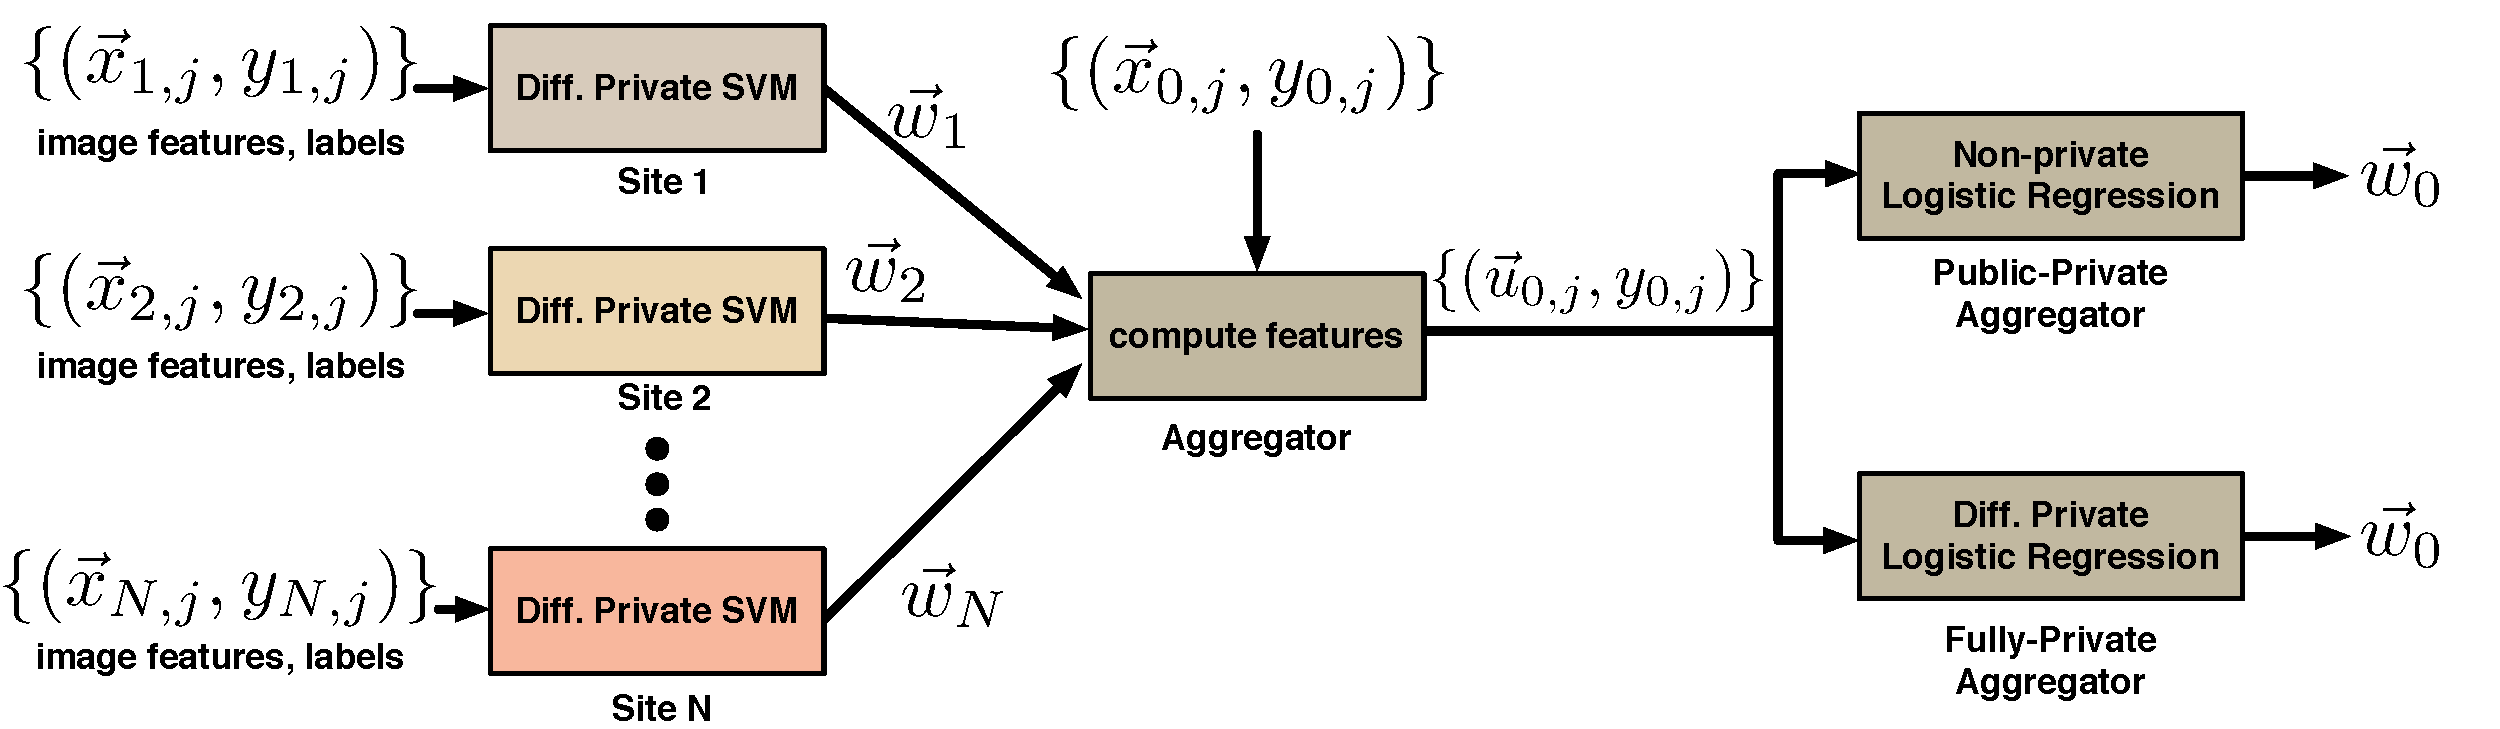
\includegraphics[width=1\linewidth]{systemfig}};
          \end{tikzpicture}
          \vskip5.5cm
        \end{block}
        
        \begin{block}{\Large Conclusions}
          \raggedright Conclude stuff here
        \end{block}
        \begin{block}{References}
          \raggedright
          \footnotesize
          \begin{thebibliography}{2}
            \raggedright
          \bibitem[Sarwate et a.(2014)]{SarwateFrontiers2014}
            Authors
            \newblock Title
            \newblock In \emph{Journal}, year.
          \end{thebibliography}
        \end{block}
      \end{column}
    \end{columns}
  \end{frame}
\end{document}


%%%%%%%%%%%%%%%%%%%%%%%%%%%%%%%%%%%%%%%%%%%%%%%%%%%%%%%%%%%%%%%%%%%%%%%%%%%%%%%%%%%%%%%%%%%%%%%%%%%%
%%% Local Variables: 
%%% mode: latex
%%% TeX-PDF-mode: t
%%% End:
